\documentclass[]{BasiliskReportMemo}
\usepackage{AVS}

\newcommand{\submiterInstitute}{Autonomous Vehicle Simulation (AVS) Laboratory,\\ University of Colorado}

\newcommand{\ModuleName}{MRP\_Steering}
\newcommand{\subject}{Nonlinear Rate Servo Feedback Control Module}
\newcommand{\status}{Initial Documentation}
\newcommand{\preparer}{H. Schaub}
\newcommand{\summary}{This module uses the MRP Steering control logic to determine the ADCS control torque vector $\bm L_{r}$.}


\begin{document}


\makeCover


%
%	enter the revision documentation here
%	to add more lines, copy the table entry and the \hline, and paste after the current entry.
%
\pagestyle{empty}
{\renewcommand{\arraystretch}{2}
\noindent
\begin{longtable}{|p{0.5in}|p{4.5in}|p{1.14in}|}
\hline
{\bfseries Rev}: & {\bfseries Change Description} & {\bfseries By} \\
\hline
Draft & Initial Documentation Draft & H. Schaub \\
1.0 & Changes after code review & H. Schaub \\
\hline

\end{longtable}
}

\newpage
\setcounter{page}{1}
\pagestyle{fancy}

\tableofcontents
~\\ \hrule ~\\

\begin{figure}[htb]
	\centerline{
	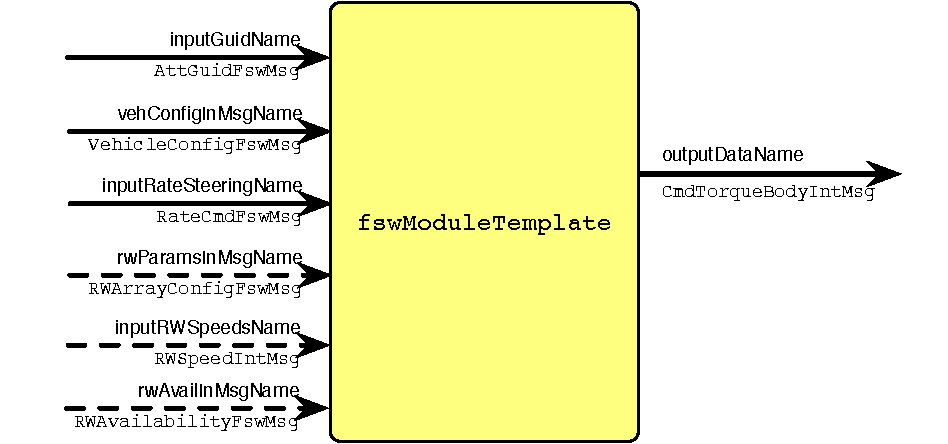
\includegraphics[]{Figures/moduleImg}
	}
	\caption{{\tt reateServoFullNonlinear} Module I/O Illustration}
	\label{fig:moduleImg}
\end{figure}
\section{Overview}
This module computes a commanded control torque vector $\bm L_r$ using a rate based steering law that drives a body frame \frameDefinition{B} towards a time varying reference frame \frameDefinition{R}, based on a desired reference frame \frameDefinition{B*} (the desired body frame from the kinematic steering law).

The module input messages  and output message are illustrated in Figure~\ref{fig:moduleImg}. The output message is a body-frame control torque vector that is outlined in section 3, with $\bm L_r$ specifically computed in equation \ref{eq:MS:39}.
 The required attitude guidance message contains both attitude tracking error rates as well as reference frame rates. This message is read in with every update cycle. The vehicle configuration message is only read in on reset and contains the spacecraft inertia tensor about the vehicle's center of mass location.  The commanded body rates are read in from the steering module output message.  
 
 The reaction wheel (RW) configuration message is optional.  If the message name is specified, then the RW message is read in.  If the optional RW availability message is present, then the control will only use the RWs that are marked available.  

The servo rate feedback control can compensate for Reaction Wheel (RW) gyroscopic effects as well. This is an optional input message where the RW configuration array message contains the RW spin axis $\hat{g}_{s,i}$ information and the RW polar inertia about the spin axis IWs,i . This is only read in on reset. The RW speed message contains the RW speed $\Omega_i$ and is read in every time step. The optional RW availability message can be used to include or not include RWs in the MRP feedback. This allows the module to selectively turn off some RWs. The default is that all RWs are operational and are included.

\section{Initialization}
Simply call the module reset function prior to using this control module.  This will reset the prior function call time variable, and reset the rotational rate error integral measure.  The control update period $\Delta t$ is evaluated automatically.  


\section{Steering Law Goals}
This technical note develops a rate based steering law that drives a body frame \frameDefinition{B} towards a time varying reference frame \frameDefinition{R}. The inertial frame is given by \frameDefinition{N}.   The RW coordinate frame is given by $\mathcal{W_{i}}:\{ \hat{\bm g}_{s_{i}}, \hat{\bm g}_{t_{i}}, \hat{\bm g}_{g_{i}} \}$.  Using MRPs, the overall control goal is 
\begin{equation}
	\label{eq:MS:1}
	\bm\sigma_{\mathcal{B}/\mathcal{R}} \rightarrow 0
\end{equation}
The reference frame orientation $\bm \sigma_{\mathcal{R}/\mathcal{N}}$, angular velocity $\bm\omega_{\mathcal{R}/\mathcal{N}}$ and inertial angular acceleration $\dot{\bm \omega}_{\mathcal{R}/\mathcal{N}}$ are assumed to be known. 

The rotational equations of motion of a rigid spacecraft with $N$ Reaction Wheels (RWs) attached are given by\cite{schaub}
\begin{equation}
	\label{eq:MS:2}
	[I_{RW}] \dot{\bm \omega} = - [\tilde{\bm \omega}] \left( 
	[I_{RW}] \bm\omega + [G_{s}] \bm h_{s} 
	\right) - [G_{s}] \bm u_{s} + \bm L
\end{equation}
where  the inertia tensor $[I_{RW}]$ is defined as
\begin{equation}
	\label{eq:MS:3}
	[I_{RW}] = [I_{s}] + \sum_{i=1}^{N} \left (J_{t_{i}} \hat{\bm g}_{t_{i}} \hat{\bm g}_{t_{i}}^{T} + J_{g_{i}} \hat{\bm g}_{g_{i}} \hat{\bm g}_{g_{i}}^{T}
	\right)
\end{equation}
The spacecraft inertial without the $N$ RWs is $[I_{s}]$, while $J_{s_{i}}$, $J_{t_{i}}$ and $J_{g_{i}}$ are the RW inertias about the body fixed RW axis $\hat{\bm g}_{s_{i}}$ (RW spin axis), $\hat{\bm g}_{t_{i}}$ and $\hat{\bm g}_{g_{i}}$.  The $3\times N$ projection matrix $[G_{s}]$ is then defined as
\begin{equation}
	\label{eq:MS:4}
	[G_{s}] = \begin{bmatrix}
		\cdots \leftexp{B}{\hat{\bm g}}_{s_{i}} \cdots
	\end{bmatrix}
\end{equation}
The RW inertial angular momentum vector $\bm h_{s}$ is defined as
\begin{equation}
	\label{eq:MS:5}
	h_{s_{i}} = J_{s_{i}} (\omega_{s_{i}} + \Omega_{i})
\end{equation}
Here $\Omega_{i}$ is the $i^{\text{th}}$ RW spin relative to the spacecraft, and the body angular velocity is written in terms of body and RW frame components as
\begin{equation}
	\label{eq:MS:6}
	\bm\omega = \omega_{1} \hat{\bm b}_{1} + \omega_{2} \hat{\bm b}_{2} + \omega_{3} \hat{\bm b}_{3}
	= \omega_{s_{i}} \hat{\bm g}_{s_{i}} +  \omega_{t_{i}} \hat{\bm g}_{t_{i}} +  \omega_{g_{i}} \hat{\bm g}_{g_{i}}
\end{equation}











\section{Angular Velocity Servo Sub-System}
To implement the kinematic steering control, a servo sub-system must be included which will produce the required torques to make the actual body rates track the desired body rates.  The angular velocity tracking error vector is defined as
\begin{equation}
	\label{eq:MS:32}
	\delta \bm \omega = \bm\omega_{\mathcal{B}/\mathcal{B}^{\ast}} = \bm\omega_{\mathcal{B}/\mathcal{N}} - \bm\omega_{\mathcal{B}^{\ast}/\mathcal{N}}
\end{equation}
where the $\mathcal{B}^{\ast}$ frame is the desired body frame from the kinematic steering law.  Note that
\begin{equation}
	 \bm\omega_{\mathcal{B}^{\ast}/\mathcal{N}} =  \bm\omega_{\mathcal{B}^{\ast}/\mathcal{R}} +  \bm\omega_{\mathcal{R}/\mathcal{N}}
\end{equation}
where $\bm\omega_{\mathcal{R}/\mathcal{N}}$ is obtained from the attitude navigation solution, and $ \bm\omega_{\mathcal{B}^{\ast}/\mathcal{R}}$ is the kinematic steering rate command.  To create a rate-servo system that is robust to unmodeld torque biases, the state $\bm z$ is defined as:
\begin{equation}
	\label{eq:MS:34}
	\bm z = \int_{t_{0}}^{t_{f}} \leftexp{B}{ \delta\bm\omega}\ \D t
\end{equation}

The rate servo Lyapunov function is defined as 
\begin{equation}
	\label{eq:MS:35}
	V_{\bm\omega}(\delta\bm\omega, \bm z) = \frac{1}{2} \delta\bm\omega ^{T} [I_{\text{RW}}] \delta\bm\omega + \frac{1}{2} \bm z ^{T} [K_{I}] \bm z
\end{equation}
where the vector $\delta\bm\omega$ and tensor $[I_{\text{RW}}]$ are assumed to be given in body frame components, $[K_{i}]$ is a symmetric positive definite matrix.  The time derivative of this Lyapunov function is
\begin{equation}
	\label{eq:MS:36}
	\dot V_{\bm\omega} = \delta\bm\omega^{T} \left(
		[I_{\text{RW}}] \delta\bm\omega' + [K_{I}] \bm z
	\right)
\end{equation}
Using the identities ${\bm\omega}_{\mathcal{B}/\mathcal{N}}' = \dot{\bm\omega}_{\mathcal{B}/\mathcal{N}}$ and $ \bm\omega_{\mathcal{R}/\mathcal{N}}' =  \dot{\bm\omega}_{\mathcal{R}/\mathcal{N}} -  {\bm\omega}_{\mathcal{B}/\mathcal{N}} \times  \bm\omega_{\mathcal{R}/\mathcal{N}}$,\cite{schaub} the body frame derivative of $\delta \bm\omega$ is
\begin{equation}
	\label{eq:MS:37}
	\delta\bm \omega '= \dot{\bm\omega}_{\mathcal{B}/\mathcal{N}} - \bm\omega_{\mathcal{B}^{\ast}/\mathcal{R}} ' -  \dot{\bm\omega}_{\mathcal{R}/\mathcal{N}} +  {\bm\omega}_{\mathcal{B}/\mathcal{N}} \times  \bm\omega_{\mathcal{R}/\mathcal{N}}
\end{equation}
Substituting Eqs.~\eqref{eq:MS:2} and \eqref{eq:MS:37} into the $\dot V_{\bm\omega}$ expression in Eq.~\eqref{eq:MS:36} yields
\begin{multline}
	\label{eq:MS:38}
	\dot V_{\bm\omega} = \delta\bm\omega^{T} \Big(
		- [\tilde{\bm \omega}_{\mathcal{B}/\mathcal{N}}] \left( 
	[I_{RW}] \bm\omega_{\mathcal{B}/\mathcal{N}} + [G_{s}] \bm h_{s} 
	\right) - [G_{s}] \bm u_{s} + \bm L + [K_{I}] \bm z
	\\
	- [I_{\text{RW}}](\bm\omega_{\mathcal{B}^{\ast}/\mathcal{R}} ' +  \dot{\bm\omega}_{\mathcal{R}/\mathcal{N}} - {\bm\omega}_{\mathcal{B}/\mathcal{N}} \times  \bm\omega_{\mathcal{R}/\mathcal{N}})
	\Big)
\end{multline}

%\begin{equation}
%	\label{eq:MS:39}
%	\dot V_{\bm\omega} = - \delta\bm\omega^{T} [P]\delta\bm\omega
%\end{equation}
Let $[P]^{T} = [P]>$ be a symmetric positive definite rate feedback gain matrix.  The servo rate feedback control is defined as
\begin{multline}
	\label{eq:MS:39}
	[G_{s}]\bm u_{s} = [P]\delta\bm\omega + [K_{I}]\bm z - [\tilde{\bm\omega}_{\mathcal{B}^{\ast}/\mathcal{N}}] 
	\left( [I_{\text{RW}}] \bm\omega_{\mathcal{B}/\mathcal{N}} + [G_{s}] \bm h_{s} \right)
	\\
	- [I_{\text{RW}}](\bm\omega_{\mathcal{B}^{\ast}/\mathcal{R}} ' +  \dot{\bm\omega}_{\mathcal{R}/\mathcal{N}} -  {\bm\omega}_{\mathcal{B}/\mathcal{N}} \times  \bm\omega_{\mathcal{R}/\mathcal{N}}) + \bm L
\end{multline}
Defining the right-hand-side as $\bm L_{r}$, this is rewritten in compact form as
\begin{equation}
	[G_{s}]\bm u_{s} = -\bm L_{r}
\end{equation}
The array of RW motor torques can be solved with the typical minimum norm inverse
\begin{equation}
	\bm u_{s} = [G_{s}]^{T}\left( [G_{s}][G_{s}]^{T}\right)^{-1} (- \bm L_{r})
\end{equation}


To analyze the stability of this rate servo control, the $[G_{s}]\bm u_{s}$ expression in Eq.~\eqref{eq:MS:39} is substituted into the Lyapunov rate expression in Eq.~\eqref{eq:MS:38}.
\begin{align}
	\label{eq:MS:42}
	\dot V_{\omega} &= \delta\bm\omega^{T} \Big(
		- [P]\delta\bm\omega - [\tilde{\bm \omega}_{\mathcal{B}/\mathcal{N}}] \left( 
	[I_{RW}] \bm\omega_{\mathcal{B}/\mathcal{N}} + [G_{s}] \bm h_{s} 
	\right) 
	+ [\tilde{\bm\omega}_{\mathcal{B}^{\ast}/\mathcal{N}}] 
	\left( [I_{\text{RW}}] \bm\omega_{\mathcal{B}/\mathcal{N}} + [G_{s}] \bm h_{s} \right)
	\Big ) 
	\nonumber \\
	&= \delta\bm\omega^{T} \Big( - [P]\delta\bm\omega
	- [\widetilde{\delta\bm \omega}] \left( 
	[I_{RW}] \bm\omega_{\mathcal{B}/\mathcal{N}} + [G_{s}] \bm h_{s} 
	\right) 
	\Big )
	\nonumber \\
	&= - \delta\bm\omega ^{T} [P] \delta\bm\omega < 0
\end{align}
Thus, in the absence of unmodeled torques, the servo control in Eq.~\eqref{eq:MS:39} is asymptotically stabilizing in rate tracking error $\delta\bm\omega$.  

Next, the servo robustness to unmodeled external torques is investigated.  Let us assume that the external torque vector $\bm L$ in Eq.~\eqref{eq:MS:2} only approximates the true external torque, and the unmodeled component is given by $\Delta \bm L$.  Substituting the true equations of motion and the same servo control in Eq.~\eqref{eq:MS:39} into the Lyapunov rate expression in Eq.~\eqref{eq:MS:36} leads to
\begin{equation}
	\label{eq:MS:43}
	\dot V_{\omega} = - \delta\bm\omega ^{T} [P] \delta\bm\omega - \delta\bm\omega ^{T} \Delta \bm L
\end{equation}
This $\dot V_{\omega}$ is no longer negative definite due to the underdetermined sign of the $\delta\bm\omega ^{T} \Delta \bm L$ components.  Equating the Lyapunov rates in Eqs.~\eqref{eq:MS:36} and \eqref{eq:MS:43} yields the following servo closed loop dynamics:
\begin{equation}
	\label{eq:MS:44}
	[I_{\text{RW}}]\delta\bm\omega' + [P]\delta\bm\omega + [K_{I}]\bm z = \Delta\bm L
\end{equation}
Assuming that $\Delta\bm L$ is either constant as seen by the body frame, or at least varies slowly, then taking a body-frame time derivative of Eq.~\eqref{eq:MS:44} is
\begin{equation}
	\label{eq:MS:45}
	[I_{\text{RW}}]\delta\bm\omega'' + [P]\delta\bm\omega' + [K_{I}]\delta \bm \omega = \Delta\bm L' \approx 0 	
\end{equation}
As $[I_{\text{RW}}]$, $[P]$ and $[K_{I}]$ are all symmetric positive definite matrices, these linear differential equations are stable, and $\delta\bm\omega\rightarrow0$ given that assumption that $\Delta\bm L' \approx 0$.  


\section{Unit Test}
The unit test for this module \verb|test_MRP_feedback| tests a set of gains $K,K_i,P$ on a rigid body with no external torques, and with a fixed input reference attitude message. The torque requested by the controller is evaluated against python computed torques at 0s, 0.5s, 1s, 1.5s and 2s to within a tolerance of $10^{-8}$. After 1s the simulation is stopped and the Reset() function is called to check that integral feedback related variables are properly reset.  The following permutations are run:
\begin{itemize}
	\item The test is run for a case with error integration feedback ($k_i=0.01$) and one case where $k_i$ is set to a negative value, resulting in a case with no integrator. 
	\item The RW array number is configured either to 4 or 0
	\item The integral limit term is set to either 0 or 20
	\item The RW availability message is tested in 3 manners.  Either the availability  message is not written where all wheels should default to being available.  If the availability message is written, then the RWs are either zero to available or not available.
	\item The values of $^B\omega'_{B^*R}$ and$^B\omega_{B^*R}$ are varied between a non-zero 3x1 vector to a zero vector
\end{itemize}
All permutations of these test cases are expected to pass.


\section{User Guide}
This module requires the following variables:
\begin{itemize}
\item $^B\mathbf{\omega}_{BR}$  as \verb|guidCmdData.omega_BR_B|
\item $^B\mathbf{\omega}_{RN}$ as \verb|guidCmdData.omega_RN_B|
\item $^B\dot{\mathbf{\omega}}_{RN}$ as \verb|guidCmdData.domega_RN_B|
\item $[I]$, the inertia matrix of the body as \verb|vehicleConfigOut.ISCPntB_B|
\item $\Omega_i$, speed of each reaction wheel in \verb|rwSpeedMessage.wheelSpeeds|
\item Gains $k,P$ in \verb|moduleConfig|. 
\item The integral gain $K_i$ in \verb|moduleConfig|. Setting this variable to a negative number disables the error integration for the controller, leaving just PI terms. 
\item The value of \verb|integralLimit|, used to limit the degree of integrator windup and reduce the chance of controller saturation. The integrator is required to maintain asymptotic tracking in the presence of an external disturbing torque. For this module, the integration limit is applied to each element of the integrated error vector $z$, and any elements greater than the limit are set to the limit instead.
\item Commanded body rates omegap\_BastR\_B and omega\_BastR\_B

\end{itemize}



\bibliographystyle{unsrt}   % Number the references.
\bibliography{references}   % Use references.bib to resolve the labels.




\end{document}
